De Unix-wereld houdt erg van het paradigma ``Small is beautiful''. Daarmee bedoelen ze dat ze
graag kleine tools maken die \'e\'en ding goed doen. Dat zien we ook terug bij de grafische interface\index{Grafische Interface}. Allereerst is er
een display server, dit is een stuk software dat ervoor zorgt dat er een grafische interface is. Het luistert naar de
muis, bestuurt de cursor en toont een grafisch scherm en dat is het wel zo'n beetje. Op deze grafische server\index{Grafische server}
draait een window-manager\index{Window-manager}. De window-manager vangt een applicatie in een frame (een window) en zorgt ervoor dat er naar
wens scrol-knoppen zijn en knopjes om het scherm te minimaliseren en/of te sluiten. Ook het achtergrondscherm is een
taak van de window-manager. Als laatste is er de desktop\index{Desktop} omgeving die zorgt voor de taakbalk, het configuratiescherm en
alle andere zaken die nodig zijn om van een desktop te kunnen spreken.

{\selectlanguage{dutch}
Als we dit allemaal hebben hebben we een desktop omgeving waarbinnen applicaties kunnen draaien.}

{\selectlanguage{dutch}
Er zijn twee dominante desktop omgevingen beschikbaar op de verschillende Linux distributies en dat zijn KDE en GNOME.
Naast deze twee zijn er nog vele verschillende anderen, maar die zullen we hier niet bespreken.}

KDE\index{KDE} was, van de twee genoemde desktopomgevingen, de eerste. Het is gebaseerd op de Qt-library\index{Qt}. In
het begin was de Qt-library geen open source vandaar dat er een concurrerent project is ontstaan. Later is het met Qt
helemaal goed gekomen en nu behoort ze tot de open source gemeenschap.

{\selectlanguage{dutch}
GNOME\index{GNOME} was het concurrerende project dat gestart werd omdat Qt niet open source was. Voor GNOME tot stand kwam was er een
open source fotomanipulatie applicatie dat The \index{GIMP}GIMP heet, zie later in dit hoofdstuk. Om het pakket te kunnen
maken hadden de ontwikkelaars een grafische library ontwikkeld die GTK\index{GTK} werd genoemd. Veel van wat er nodig is voor een
desktop zat daar al in en dus gebruikte het GNOME project de GTK-library als basis.}

De grafische interface kan enorm verschillen per distributie. Het maakt al enorm veel verschil
of je KDE of GNOME gebruikt als desktop omgeving. Laat je hierdoor niet imponeren, het wijst zich vaak vanzelf. KDE
ligt qua interface het dichtst tegen Windows aan, en zal dus het makkelijkst zijn om naar over te stappen. CentOS
gebruikt GNOME en vergt iets meer doorzettingsvermogen om te doorgronden.

Mocht het scherm in zijn screensaver\index{Screensaver!Login} vallen dan kan je door klikken met de muis een scherm krijgen waarop
de tijd te zien is, daarna kom je met de {\textless}Enter{\textgreater} toets op een login scherm en kan je in loggen met je
gebruikersnaam en wachtwoord.

Eenmaal ingelogd kan je door op Activities\index{Activities} te klikken extra scherm elementen te zien krijgen (zie figuur \ref{fig:de_activities}). Het nog een keer
aanklikken van Activities verbergt de elementen weer waardoor je meer ruimte op je desktop hebt voor applicaties (zie figuur \ref{fig:de_deactivities}).

\begin{figure}[H]
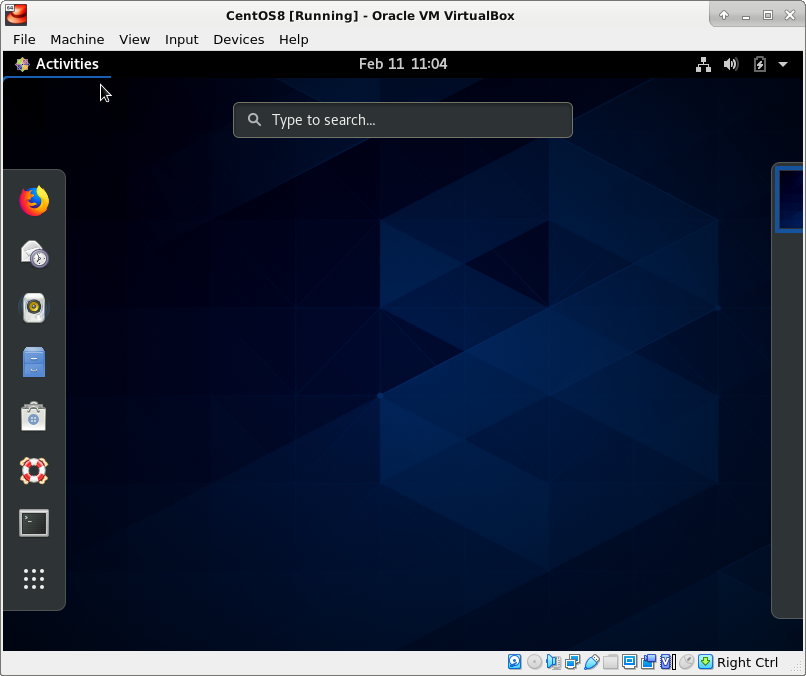
\includegraphics[width=0.9\textwidth]{linuxreader-img013.png}
	\caption{De desktop met alle scherm elementen}
	\label{fig:de_activities}
\end{figure}
\begin{figure}[H]
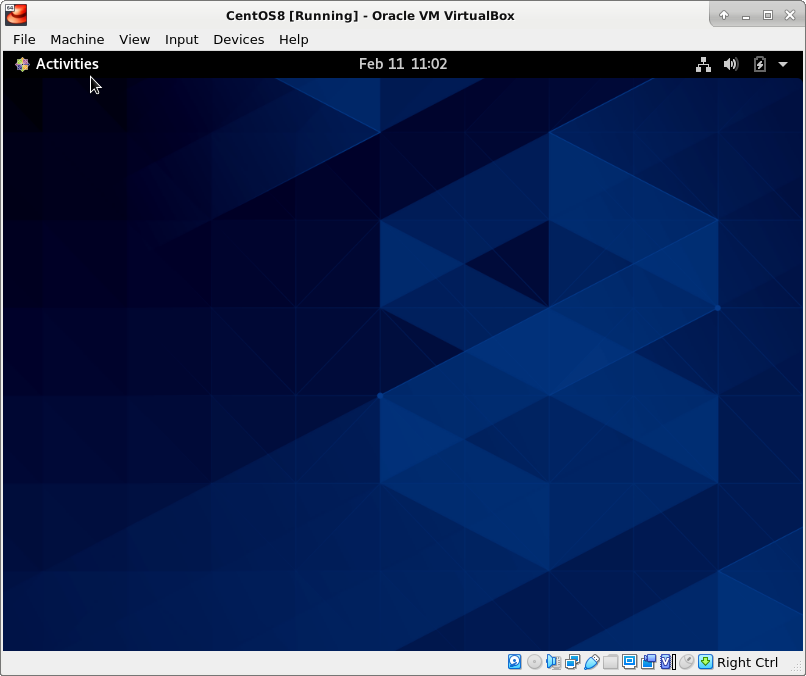
\includegraphics[width=0.9\textwidth]{linuxreader-img014.png}
	\caption{De desktop zonder alle scherm elementen}
	\label{fig:de_deactivities}
\end{figure}
